\appendix

\begin{graphicspathcontext}{{./chapters/appendix/imgs/auto/}{./chapters/appendix/imgs/raw/}}
	
\section{Document License}
\sectiontableofcontentslide

\begin{frame}[t]{{Creative Common License} CC-BY-NC-SA 3.0}
	\begin{center}\footnotesize
	``\inserttitle'' by \insertauthor\ is licensed under a Creative Commons Attribution-NonCommercial-ShareAlike 3.0 Unported License.
	\end{center}
	\begin{block}{\footnotesize You are free}\scriptsize
		\begin{tabularx}{\linewidth}{m{.04\linewidth}@{\hspace{.5em}}lX}
		\raisebox{-.5\height}{
\includegraphics[width=\linewidth]{creative_toshare}} &
		\Emph{To Share} & to copy, distribute and transmit the work \\
		\raisebox{-.5\height}{
\includegraphics[width=\linewidth]{creative_toremix}} &
		\Emph{To Remix} & to adapt the work \\
		\end{tabularx}
	\end{block}
	\vspace{.25cm}
	\begin{block}{\footnotesize Under the following conditions}\scriptsize
		\begin{tabularx}{\linewidth}{m{.04\linewidth}@{\hspace{.5em}}lX}
		\raisebox{-.5\height}{
\includegraphics[width=\linewidth]{creative_attribution}} &
		\Emph{Attribution} & You must attribute the work in the manner specified by the author or licensor (but not in any way that suggests that they endorse you or your use of the work). \\
		\raisebox{-.5\height}{
\includegraphics[width=\linewidth]{creative_noncommercial}} &
		\Emph{Noncommercial} & You may not use this work for commercial purposes. \\
		\raisebox{-.5\height}{
\includegraphics[width=\linewidth]{creative_sharealike}} &
		\Emph{Share alike} & If you alter, transform, or build upon this work, you may distribute the resulting work only under the same or similar license to this one. \\
		\end{tabularx}
	\end{block}
	\vspace{.5cm}
	\centering Greetings: icons are from The Noun Project \\
	(\url{https://thenounproject.com}) under CC license
\end{frame}

\section{Document Details}
\sectiontableofcontentslide

\begin{frame}[t]{Source and Generation Details}
	\begin{smaller}
		\begin{block}{History}
			2012-2021: Slides for the module LO46 \\
			Since 2021: Renaming LO46 to DA53
		\end{block}
		\vspace{.25cm}
		\begin{block}{Sources}
			The \LaTeX\ code of this document is available at \url{https://github.com/gallandarakhneorg/da53-lessons}
		\end{block}
		\vspace{.25cm}
		\begin{block}{Generation}
			This document is generated \today\ with the following tools:
			\begin{itemize}
			\item \LaTeX
			\item Beamer
			\item CIAD style for Beamer (version \insertciadbeamerthemeversion) --- \url{https://github.com/gallandarakhneorg/tex-templates}
			\item AutoLaTeX --- \url{http://www.arakhne.org/autolatex}
			\end{itemize}
		\end{block}
	\end{smaller}
\end{frame}

\section{About the Author and Contributors}
\sectiontableofcontentslide

\begin{frame}{{Author:} Prof\string.dr\string. St\'ephane GALLAND}
	\begin{minipage}[t]{.75\linewidth}
		\begin{raggedright}
			\textit{Full Professor} \\[.5cm]
			{\scriptsize
				Universit\'e de Technologie de Belfort-Montb\'eliard\\
				Universit\'e de Bourgogne-Franche-Comt\'e, France \\
				Deputy Director of the CIAD Laboratory} \\[.25cm]
			\textbf{Topics: Multiagent systems, Agent-based simulation, Agent-oriented software engineering, Mobility and traffic modeling} \\[.5cm]
		\end{raggedright}
	\end{minipage}%
	\hfill%
	\raisebox{-\height}{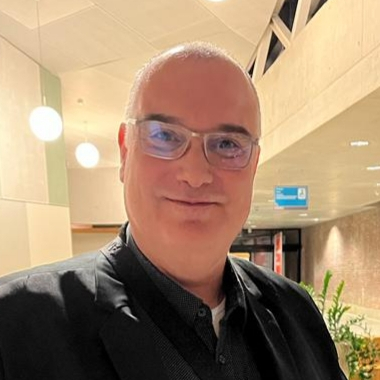
\includegraphics[width=2cm]{sgalland}} \\[.5cm]%
	\begin{raggedright}
		\scriptsize \begin{tabularx}{\linewidth}{@{}lX@{}}
			Web page: & \url{http://www.ciad-lab.fr/author-10836/} \\
			Email: & \href{mailto:stephane.galland@utbm.fr}{stephane.galland@utbm.fr} \\
		\end{tabularx} \\[.5cm]
		\scriptsize Open-source contributions:\begin{itemize}\tiny
			\item \url{http://www.sarl.io}
			\item \url{http://www.janusproject.io}
			\item \url{http://www.aspecs.org}
			\item \url{http://www.arakhne.org}
			\item \url{https://github.com/gallandarakhneorg/}
		\end{itemize}
	\end{raggedright}
\end{frame}

\begin{frame}{{Contributor \#1:} Yann LE VAGUER\`ES}
	\begin{minipage}[t]{.75\linewidth}
		\begin{raggedright}
			\textit{Computer Science Department} \\[.5cm]
			{\scriptsize
				Universit\'e de Technologie de Belfort-Montb\'eliard\\
				Universit\'e de Bourgogne-Franche-Comt\'e, France} \\[.25cm]
		\end{raggedright}
	\end{minipage}%
	\hfill%
	\raisebox{-\height}{
\includegraphics[width=1.5cm]{yann}} \\[.5cm]%
	\begin{raggedright}
		\scriptsize \begin{tabularx}{\linewidth}{@{}lX@{}}
			Web page: & \url{https://therolf.fr} \\
			Email: & \href{mailto:yann.le-vagueres@utbm.fr}{yann.le-vagueres@utbm.fr} \\
		\end{tabularx} \\[.5cm]
		\scriptsize Contributions:\begin{itemize}\tiny
			\item In this document: fixing of issues in the text and examples.
			\item Open Source: \url{https://github.com/TheRolfFR}
		\end{itemize}
	\end{raggedright}
\end{frame}

%\bibliography{biblio}

\end{graphicspathcontext}